\documentclass[digital, oneside, table, nolot, nolof]{fithesis3}
%\documentclass[printed, twoside, table, nolot, nolof]{fithesis3}

%% The following section sets up the locales used in the thesis.
\usepackage[resetfonts]{cmap}
\usepackage[T1]{fontenc}
\usepackage[main=czech, english]{babel}

%% The following section sets up the metadata of the thesis.
\thesissetup{
    date          = \the\year/\the\month/\the\day,
    university    = mu,
    faculty       = fi,
    type          = mgr,
    author        = Jan Horáček,
    gender        = m,
    advisor       = {RNDr. Zdeněk Matěj, Ph.D.},
    title         = {Návrh a implementace nového protokolu sběrnice MTBbus},
    TeXtitle      = {Návrh a implementace nového protokolu sběrnice MTBbus},
    keywords      = {sběrnice, mtb, rs485, embedded, stm32, C++, qt, protokol, avr, arm, kicad},
    TeXkeywords   = {sběrnice, mtb, rs485, embedded, stm32, C++, qt, protokol, avr, arm, kicad},
    abstract      = {Se zaváděním počítačového řízení železniční dopravy vznikaly systémy umožňující
centrálnímu řídicímu počítači interakci s~venkovními prvky zabezpečovacího
zařízení – výhybkami, návěstidly apod. Tato práce se zaměřuje na návrh
a~implementaci sběrnice, která takovou interakci umožní, ovšem na kolejištích
modelových. Práce navrhuje a~implementuje nový protokol sběrnice pro řízení
modelových kolejišť \textit{MTBbus}. Je popsáno, proč je současný systém řízení
kolejiště nedostatečný, jsou formulovány požadavky na nový systém, tento systém
je implementován. V~rámci práce vznikl detailní návrh nového protokolu, nové
hardwarové moduly pro řízení kolejiště, modul pro komunikaci s~počítačem,
obslužný počítačový software a~knihovna integrující nový hardwarový systém se
současným řídicím softwarem kolejiště.  Nový řídicí systém byl otestován
a~nasazen na skutečná kolejiště, čímž umožnil jejich další rozšiřování
a~zprovoznění nových způsobů řízení dopravy. Vznikl otevřený a~robustní systém
s~výhledem dlouhodobé udržitelnosti, který svými vlastnostmi převyšuje mnohé
současné komerční systémy řízení modelových kolejišť.  Vzniknuvší systém je
obecný, takže jej lze použít i~v~mnoha jiných aplikacích.
},
    thanks        = {Děkuji především všem, kteří ve mně zažehli, podporovali a~podporují můj velký
koníček – řízení modelové železnice. Ať už se jedná o~tátu
Miroslava, přítelkyni Verču, členy brněnského modelářského klubu nebo vedoucího
mé diplomové práce Zdeňka Matěje. Všichni ti mi umožnili psát diplomovou práci,
jejíž náplň mi dává smysl, jejíž realizace mě baví a jejíž výsledky vidím
v~reálném světě. Moc si vaší podpory vážím.
Děkuji svému vedoucímu Zdeňku Matějovi za korektury a~podporu ve změně tématu.
Děkuji konzultantovi Honzu Mrázkovi za odpovídání na mé dotazy a~za rady.
Děkuji všem korektorům této práce: Veronice Burgerové, Miroslavu Horáčkovi
a~Zdeňku Matějovi.
Děkuji mé přítelkyni Veronice a tučňákovi Adalbertovi za mentální podporu.
},
    bib           = bibliography.bib,
    titleEn       = {Design and implementation of a new MTBbus protocol},
    TeXtitleEn    = {Design and implementation of a new MTBbus protocol},
    keywordsEn    = {bus, mtb, rs485, embedded, stm32, C++, qt, protocol, avr, arm, kicad},
    TeXkeywordsEn = {bus, mtb, rs485, embedded, stm32, C++, qt, protocol, avr, arm, kicad},
    assignment    = {data/zadani_ofic.pdf},
}
\usepackage{makeidx}      %% The `makeidx` package contains
\makeindex                %% helper commands for index typesetting.
%% These additional packages are used within the document:
\usepackage{paralist} %% Compact list environments
\usepackage{amsmath}  %% Mathematics
\usepackage{amsthm}
\usepackage{amsfonts}
\usepackage{url}      %% Hyperlinks
\usepackage{listings} %% Source code highlighting
\usepackage{enumitem}
\usepackage{afterpage}
\usepackage{glossaries}
\makeglossaries
\lstset{
  basicstyle      = \ttfamily,%
  identifierstyle = \color{black},%
  keywordstyle    = \color{blue},%
  keywordstyle    = {[2]\color{cyan}},%
  keywordstyle    = {[3]\color{olive}},%
  stringstyle     = \color{teal},%
  commentstyle    = \itshape\color{magenta}}
\usepackage{floatrow} %% Putting captions above tables
\floatsetup[table]{capposition=top}
\Urlmuskip=0mu plus 1mu
\begin{document}

% Highlight overfulls
% \setlength{\overfullrule}{5pt} % TODO: remove

\setlength{\parindent}{0cm}
\setlength{\parskip}{3mm plus2pt minus2pt}
\setlist{leftmargin=8mm}
\renewenvironment{compactenum}
	{\begin{enumerate}[leftmargin=8mm,itemsep=0pt,parsep=1pt,topsep=1pt,partopsep=1pt]}
	{\end{enumerate}}
\renewenvironment{compactitem}
	{\begin{itemize}[leftmargin=8mm,itemsep=0pt,parsep=0pt,topsep=1pt,partopsep=1pt]}
	{\end{itemize}}

\newglossaryentry{plc} {
	name=PLC,
	description={Programmable Logic Controller, robustní zařízení průmyslové
	atumatizace}
}

\newglossaryentry{mtb} {
	name=MTB,
	description={Hardwarový systém pro řízení modelových kolejišť složený ze
	sběrnice MTBbus, MTB modulů a~MTB-USB desky}
}

\newglossaryentry{mtbbus} {
	name=MTBbus,
	description={Model Train Bus\footnote{Expanze zkratky do jejího plného
	významu nedává smysl, i tak budeme používat označení MTBbus, protože tak je
	zkratka zaužívaná.}, sběrnice určená pro řízení modelových kolejišť}
}

\newglossaryentry{dcc} {
	name=DCC,
	description={Digital Command Control, mezinárodně užívaný standardizovaný
	systém pro digitální řízení modelové železnice}
}

\newglossaryentry{kmz}{
	name={KMŽ Brno~I},
	description={Klub modelářů železnic Brno~I}
}

\newglossaryentry{nmra}{
	name={NMRA},
	description={National Model Railroad Association}
}

\newglossaryentry{mtbusb}{
	name={MTB-USB},
	description={Master modul sběrnice MTBbus, implementuje rozhraní mezi MTBbus
	a počítačem (USB)}
}

\newglossaryentry{mtbuni}{
	name={MTB-UNI},
	description={Nejrozšířenější slave modul sběrnice MTBbus, má 16~digitálních
	vstupů a~16~digitálních výstupů}
}

\newglossaryentry{ttl}{
	name={TTL},
	description={Transistor-transistor-logic, v~kontextu této práce standard
		definující jaká napěťová úroveň odpovídá jaké logické úrovni}
}

\newglossaryentry{usb}{
	name={USB},
	description={Universal Serial Bus, v současnosti nejpoužívanější sběrnice
	pro připojení periferií k počítači}
}

\newglossaryentry{cdc}{
	name={CDC},
	description={USB Comunications Device Class, třída USB protokolu implementující
		tunelování sériové linky skrze USB}
}

\newglossaryentry{dps}{
	name={dps},
	description={Deska plošnýcn spojů}
}

\printglossary[title=Seznam použitých zkratek]



\chapter{Úvod} \label{chap:uvod}
\textit{Programmable Logic Controller} (\gls{plc}) je vestavěný počítač, který
zpracovává vstupy, provádí jejich vyhodnocování, komunikuje s~dalšími \gls{plc}
obvody a~nastavuje výstupy \cite{plc:web}. Na rozdíl od běžných počítačů typu
\textit{PC} mají \gls{plc} větší množství vstupů a~výstupů, běží na nich
\textit{realtime} operační systémy a~jsou vysoce robustní.

\gls{plc} jsou základní jednotkou průmyslové automatizace. Používají se
například pro řízení světel dopravních křižovatek, výrobních linek, eskálátorů,
řízení elektráren, rozvoden apod. Všude tam \gls{plc} zpracovávají data z~čidel
a~ovládají periferie – například motorické pohony, signalizační diody,
robotické ruky, lasery apod.

\begin{figure}[ht]
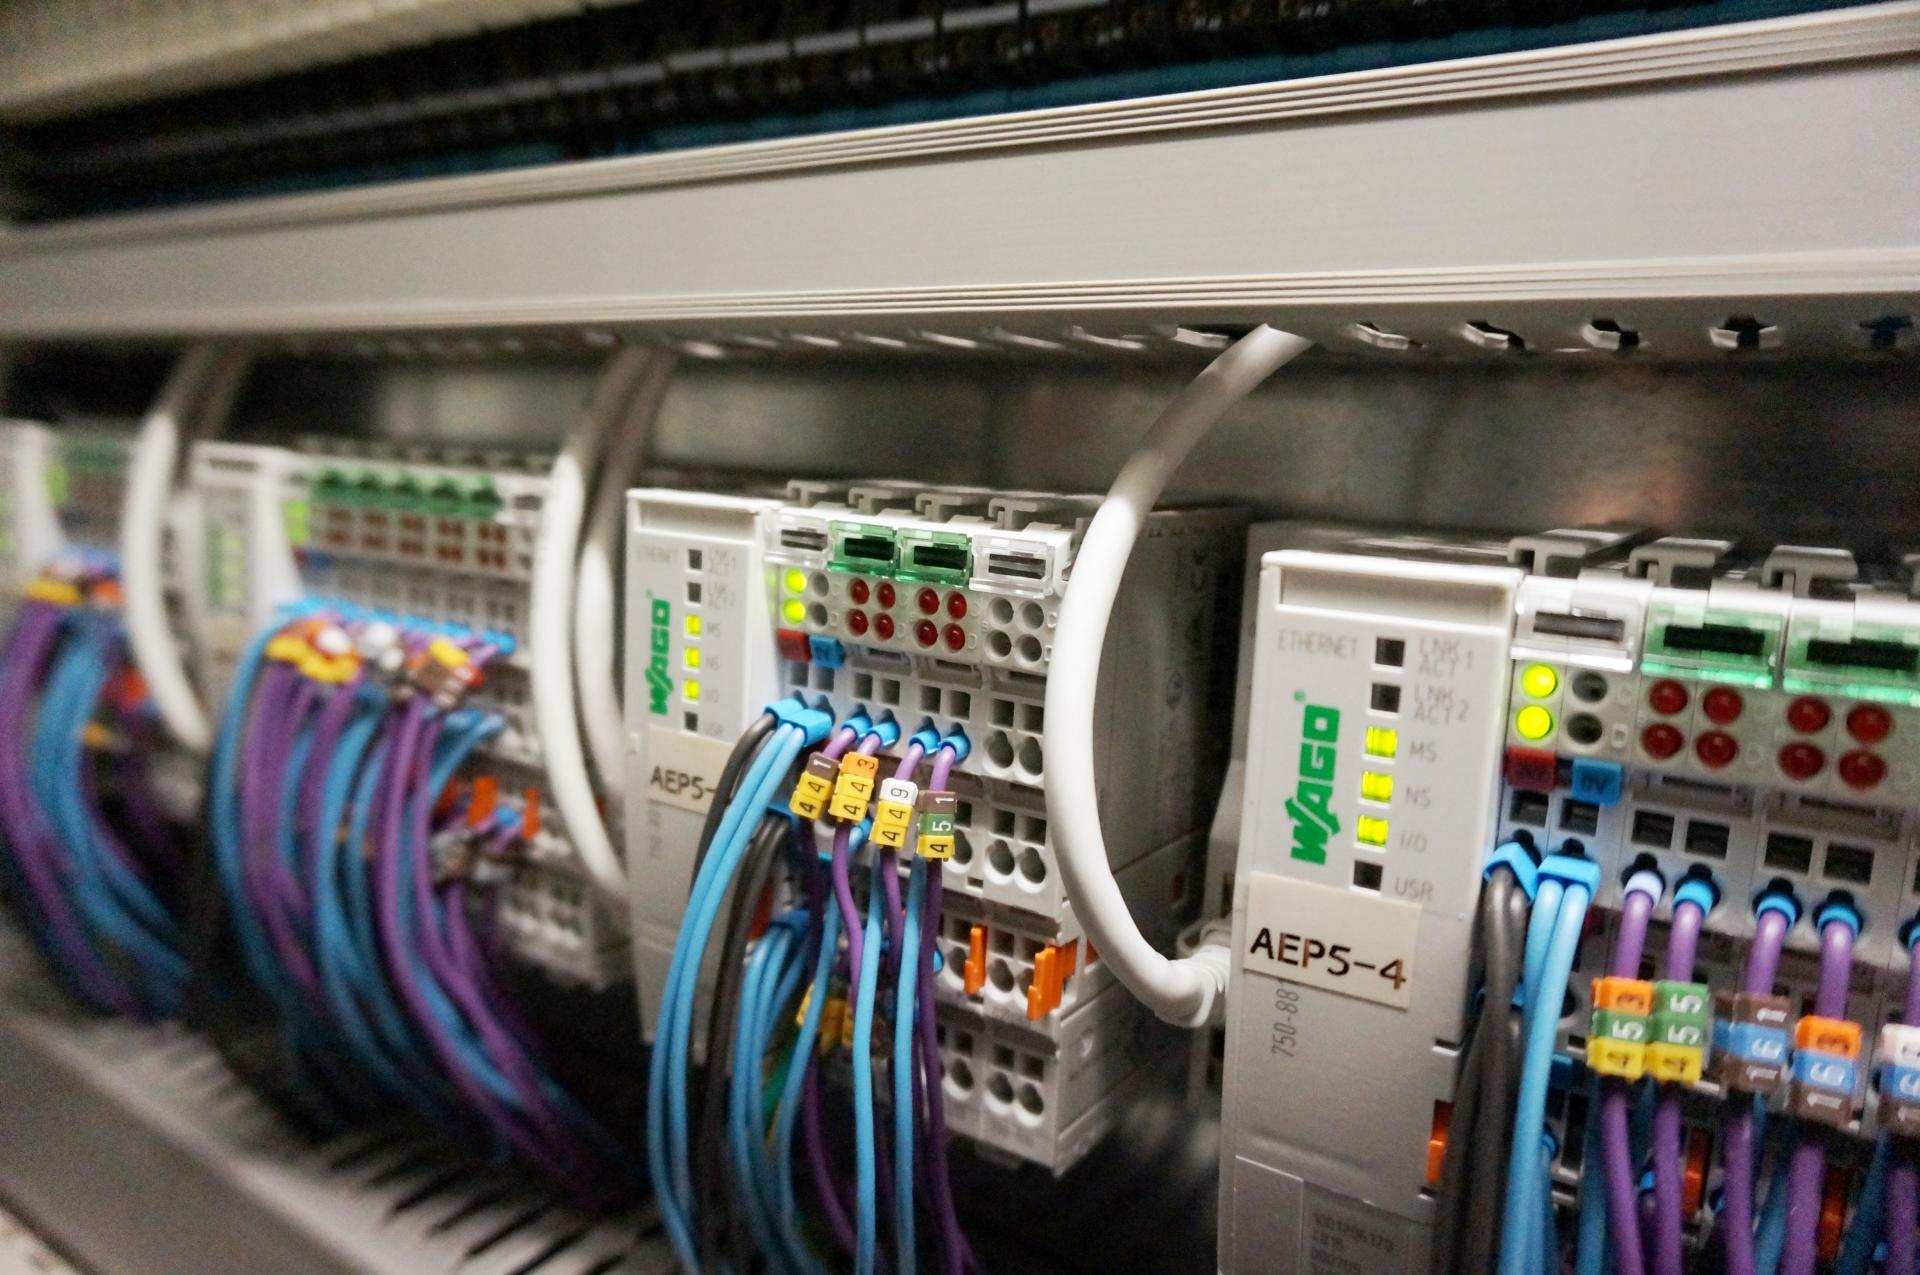
\includegraphics[width=0.7\textwidth]{data/plc.jpg}
\caption{Průmyslové \gls{plc} moduly. Převzato z~\texttt{wikimedia.org}.}
\label{fig:mtbusb-prototype}
\end{figure}

V~této práci se zaměříme na podmnožinu \gls{plc} modulů – totiž na takové,
jejichž hlavním úkolem je správně zpracovávat vstupní signály a~ovládat výstupní
periferie. Řízení logiky průmyslového procesu přenecháme počítači, s~kterým
\gls{plc} moduly komunikují.\footnote{V~praxi může \gls{plc} modul řídit logiku
procesu přímo, my však tuto situaci zkoumat nebudeme.}

Cílem této práce je navrhnout a implementovat novou verzi komunikační sběrnice
\gls{plc} obvodů \textit{\gls{mtbbus}} (\textit{Model Train
Bus}\footnote{Expanze zkratky do jejího plného významu nedává smysl, i~tak
budeme používat označení MTBbus, protože tak je zkratka zaužívaná.}).

\gls{mtbbus} je sběrnice, která se využívá pro řízení modelových kolejišť.
Je součástí systému \gls{mtb}. Skrze sběrnici lze číst signály z~kolejiště
(například polohy výhybek, obsazenost kolejových obvodů) a~povelovat prvky
v~kolejišti (návěstidla, přestavníky výhybek, přejezdy apod.). Obdobným
způsobem funguje zapezpečovací zařízení na skutečné železnici.

V~této práci autor nejprve popíše současné nasazení systému \gls{mtb}. Budou
formulovány důvody vedoucí k~nutnosti aktualizace sběrnice. Autor popíše, proč
jsou dostupná komerční řešení nevhodná a~navrhne vlastní nové (1) protokoly,
(2) hardwarové moduly a~(3) počítačové programy, které jím formulovaný problém
řeší.


\chapter{Závěr} \label{chap:zaver}
Tato diplomová práce demonstrovala, že pro vytvoření plnohodnotného \gls{plc}
systému je třeba zvládnout širokou škálu dílčích kroků. Od návrhu komunikačních
protokolů, přes návrh hardwaru, programování firmwaru, až po programování
počítačových aplikací a~knihoven. Autorovi se povedlo všechny tyto kroky
úspěšně provést. Podařilo se mu vytvořit

\begin{compactitem}
\item nový protokol \gls{mtbbus},
\item nový master modul sběrnice \gls{mtbbus} (\gls{mtbusb} v4),
\item nový univerzální \textit{slave} modul sběrnice \gls{mtbbus} (\gls{mtbuni} v4),
\item nástavný modul do starších modulů \gls{mtbuni} (MTB-2-AVR),
\item počítačovou aplikaci pro přístup k~systému \gls{mtb} (MTB Daemon),
\item knihovnu pro integraci nového \gls{mtb} do současného řídicího systému
	kolejiště (hJOP MTB Network RCS Library)
\end{compactitem}

Komponenty vytvořené v~rámci této práce a~jejich interakce jsou přehledně
zobrazeny v~\ref{fig:new-topology}.

\begin{figure}[ht]
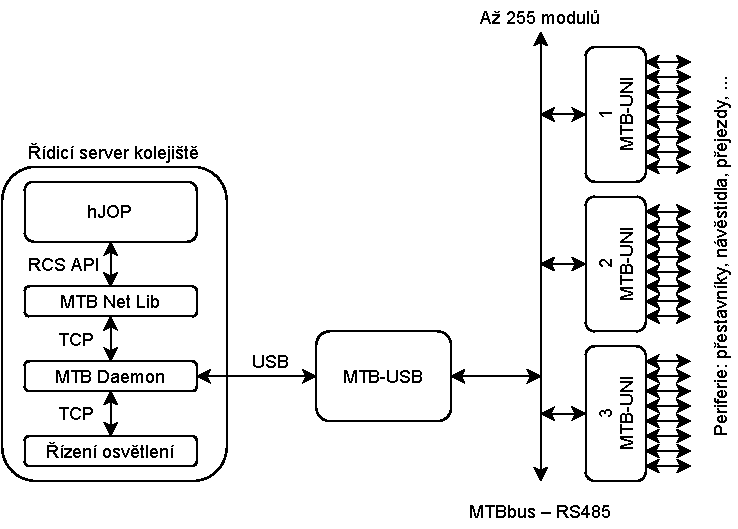
\includegraphics[width=0.8\textwidth]{data/new-topology.pdf}
\caption{Komponenty vytvořené v~rámci diplomové práce (mimo \textit{hJOP}
a~\textit{Řízení osvětlení}).}
\label{fig:new-topology}
\end{figure}

V~rámci práce byly formulovány požadavky (\ref{sub:mtbbus-req-summary}), které
má nový systém \gls{mtb} splnit. Všechny tyto požadavky byly naplněny.
Podařilo se vytvořit systém, který za poměrně malé finanční a časové náklady
značně povyšuje současný systém \gls{mtb}. Především však vznikl otevřený
a rozšiřitelný systém s~výhledem udržitelnosti po desítky let. Nový systém
\gls{mtb} umožní stavbu dalších kolejišť, udržování a rozšiřování kolejišť
současných. Nový systém \gls{mtb} si může vyrobit každý, kdo bude chtít bezpečně
řídit své modelové kolejiště.

Pro \gls{kmz} znamená \gls{mtb} v4 možnost nasadit více řídicích systémů
kolejiště, a~konečně tak zprovoznit řízení osvětlení, řízení tramvajové
a~autobusové dopravy. \gls{mtb} v4 umožní nasazení pultů obsluhy,
vytvoření nových chytrých zesilovačů \gls{dcc} signálu. Umožní výstavbu nového
depa kolejových vozidel, kde se budou používat speciální \gls{mtb} moduly.
Pro \gls{kmz} je \gls{mtb} v4 velkým krokem vpřed.

\gls{mtb} v4 bylo nasazeno na testovacím kolejišti o~20 modulech, kde úspešně
funguje.

\section{Možná rozšíření} \label{sec:future}

Při návrhu tak velkého systému, jako je \gls{mtb}, se přirozeně ukázaly mnohé
cesty, které by bylo možné v~budoucnu prozkoumat.

Systém \gls{mtb} by v~budoucnu mohl podporovat vyšší rychlosti komunikace nebo
automatickou detekci rychlosti sběrnice. \gls{mtb} by mohlo být rozšířeno
o~jednotky, které provádějí retranslaci dat sběrnice bezdrátově (pro vzdálené
připojení modulů).

Jednou z~otázek týkajících se budoucího rozšíření je, jak umožnit, aby systém
\gls{mtb} mohl interagovat s~komerčními softwary pro řízení modelových
kolejišť.
Dalším možným rozšířením je tak implementovat do majoritních komerčních
softwarů pro řízení modelových kolejišť podporu pro \gls{mtb}. Některé softwary
jsou však uzavřené. Pro takové softwary by bylo možné napsat alternativní
firmware do \gls{mtbusb}, který by zajistil, že \gls{mtbusb} modul se pro
počítač bude tvářit jako některý z~komerčních systémů pro řízení kolejišť.

Dalším přirozeným způsobem rozšíření, který má autor této práce v~plánu
v~nejbližším roce uskutečnit, je přidání dalších typů modulů. V~budoucnu
vzniknou \gls{mtb} moduly pro chytré zesilovače \gls{dcc} signálu,
\textit{RailCom} detektory a jiné. Systém \gls{mtb} je na tato rozšíření
připraven.


\printbibliography[heading=bibintoc]

\appendix
\chapter{Přílohy} \label{chap:appendix}
\vspace{-2em}

\begin{figure}[H]
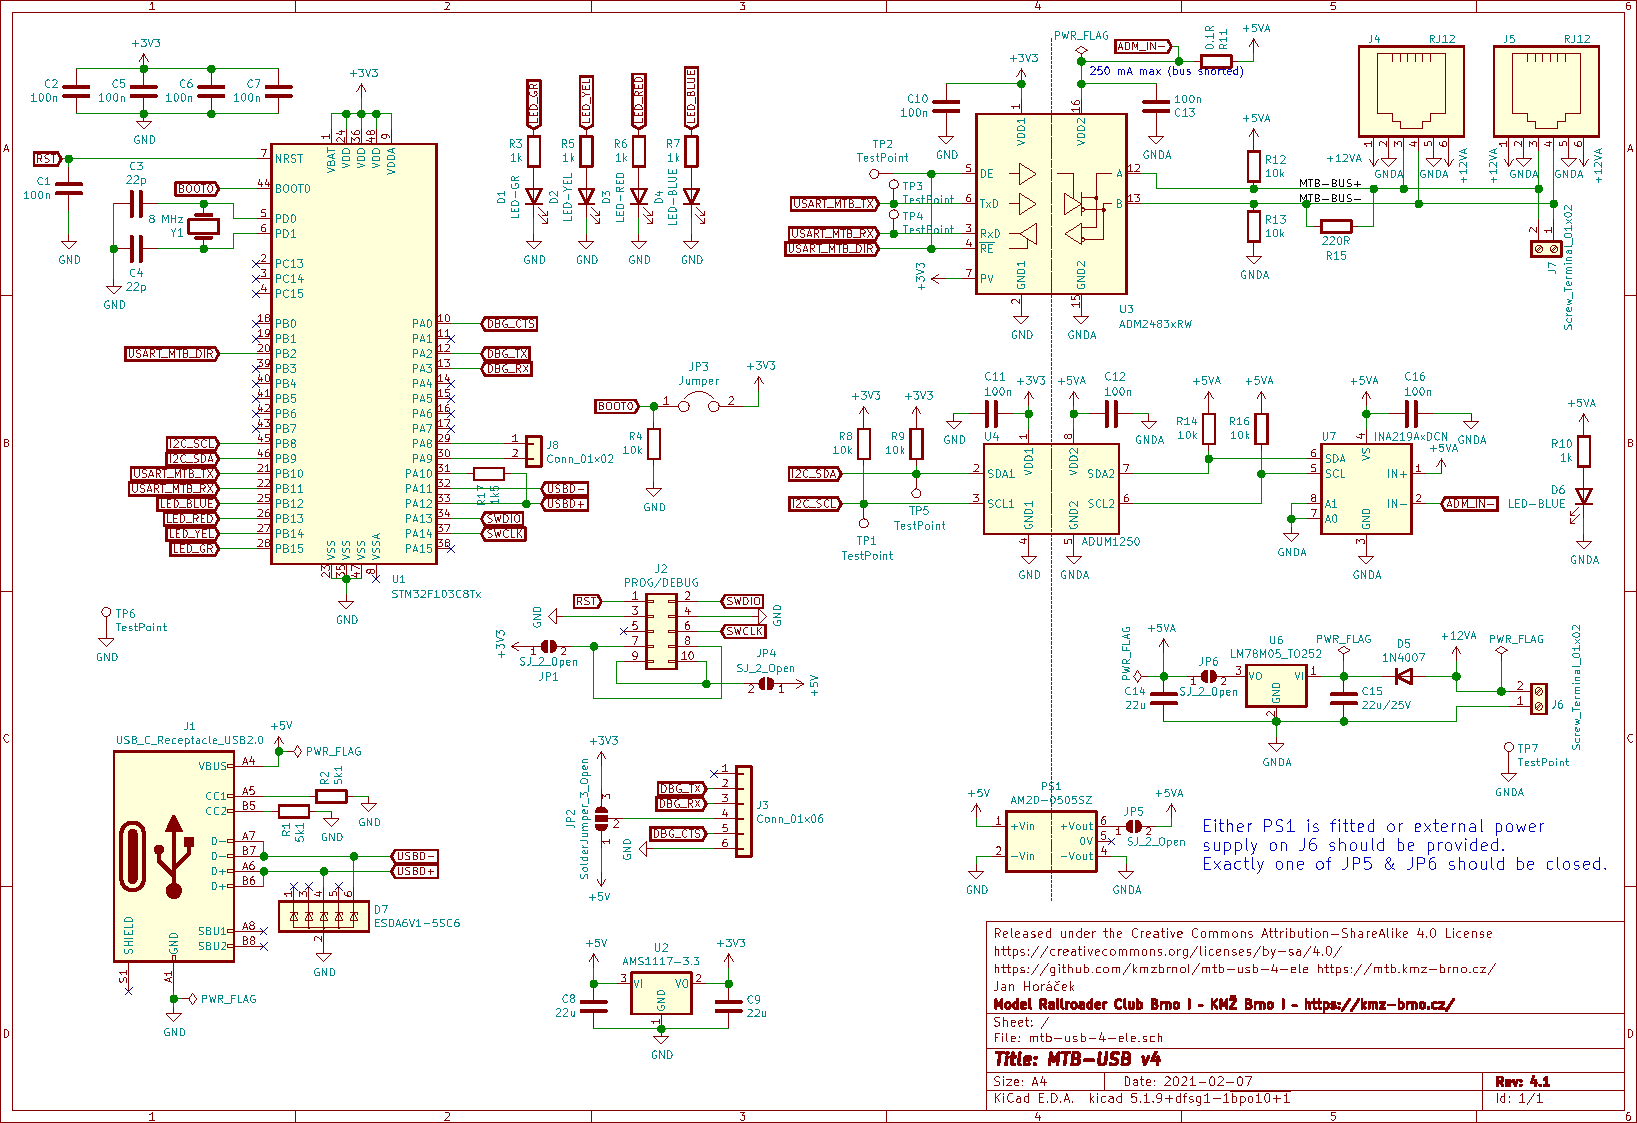
\includegraphics[angle=90,width=\textwidth]{data/mtb-usb-4-ele.pdf}
\caption{Schéma \gls{mtbusb} modulu.}
\label{fig:mtb-usb-sch}
\end{figure}

\begin{figure}[ht]
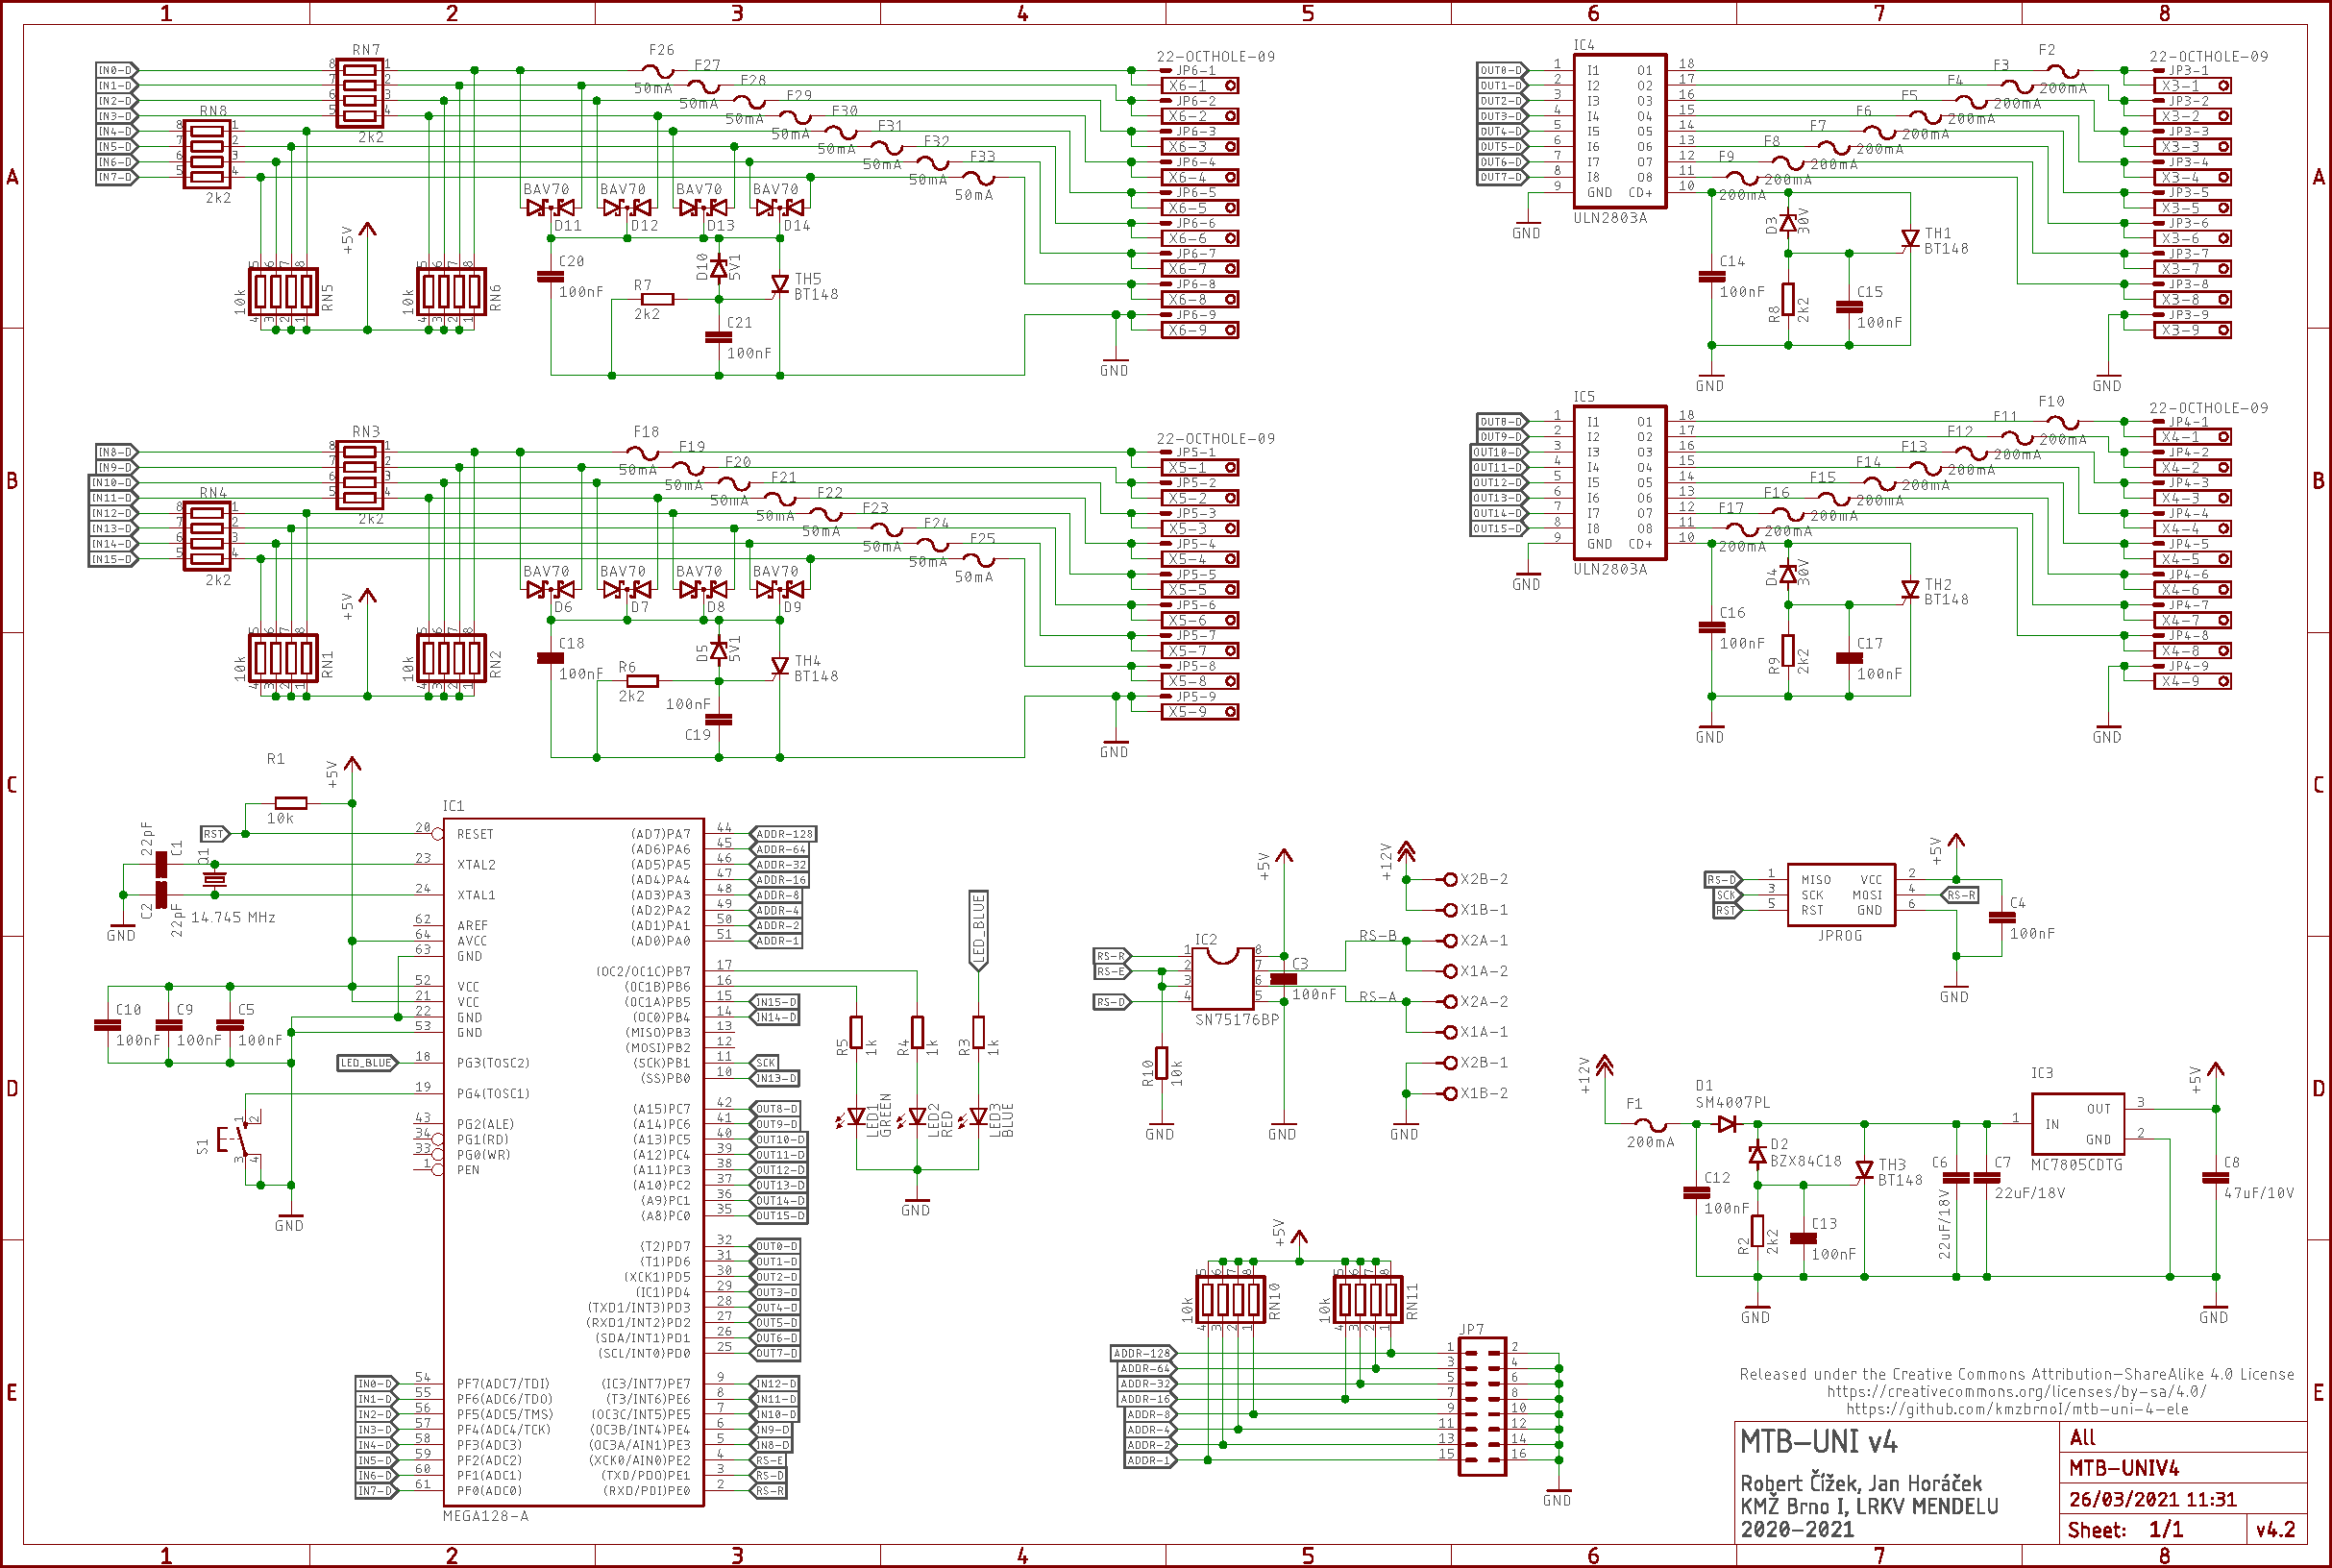
\includegraphics[angle=90,width=\textwidth]{data/mtb-uni-4-ele.pdf}
\caption{Schéma \gls{mtbuni} v4 modulu.}
\label{fig:mtb-uni-4-sch}
\end{figure}

\begin{figure}[ht]
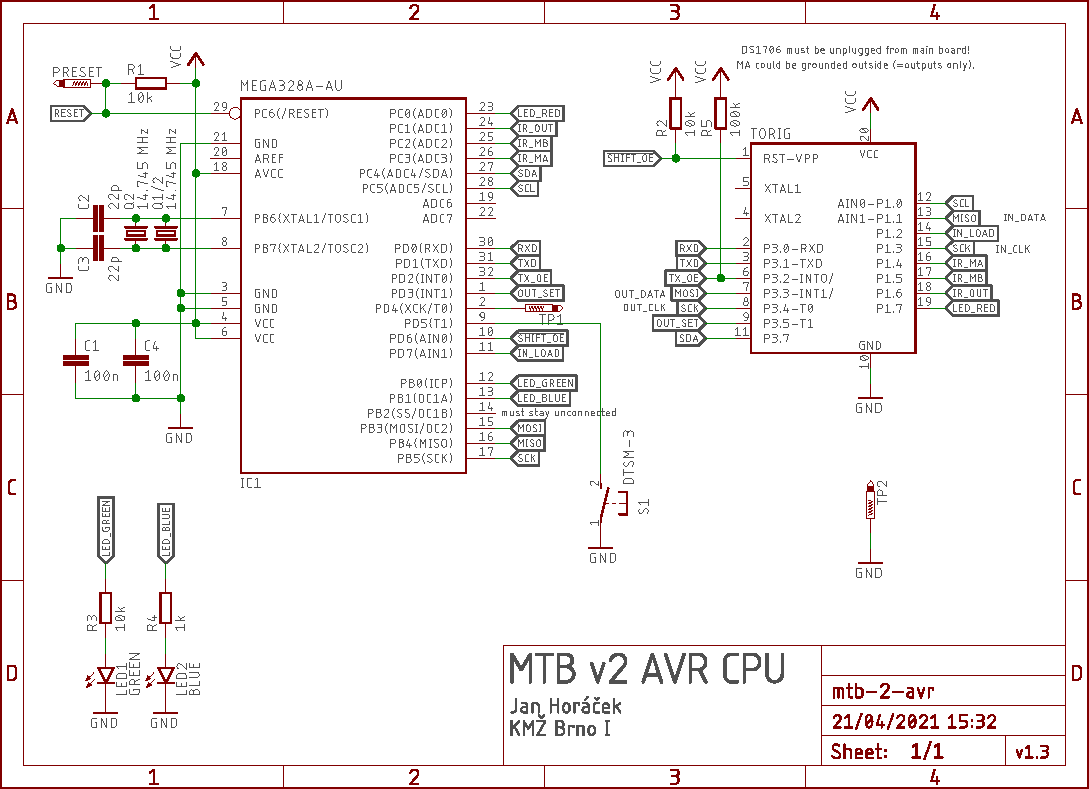
\includegraphics[angle=90,width=\textwidth]{data/mtb-2-avr-ele.pdf}
\caption{Schéma nástavné desky \textit{MTB-2-AVR}.}
\label{fig:mtb-uni-2-avr-sch}
\end{figure}

\begin{figure}[ht]
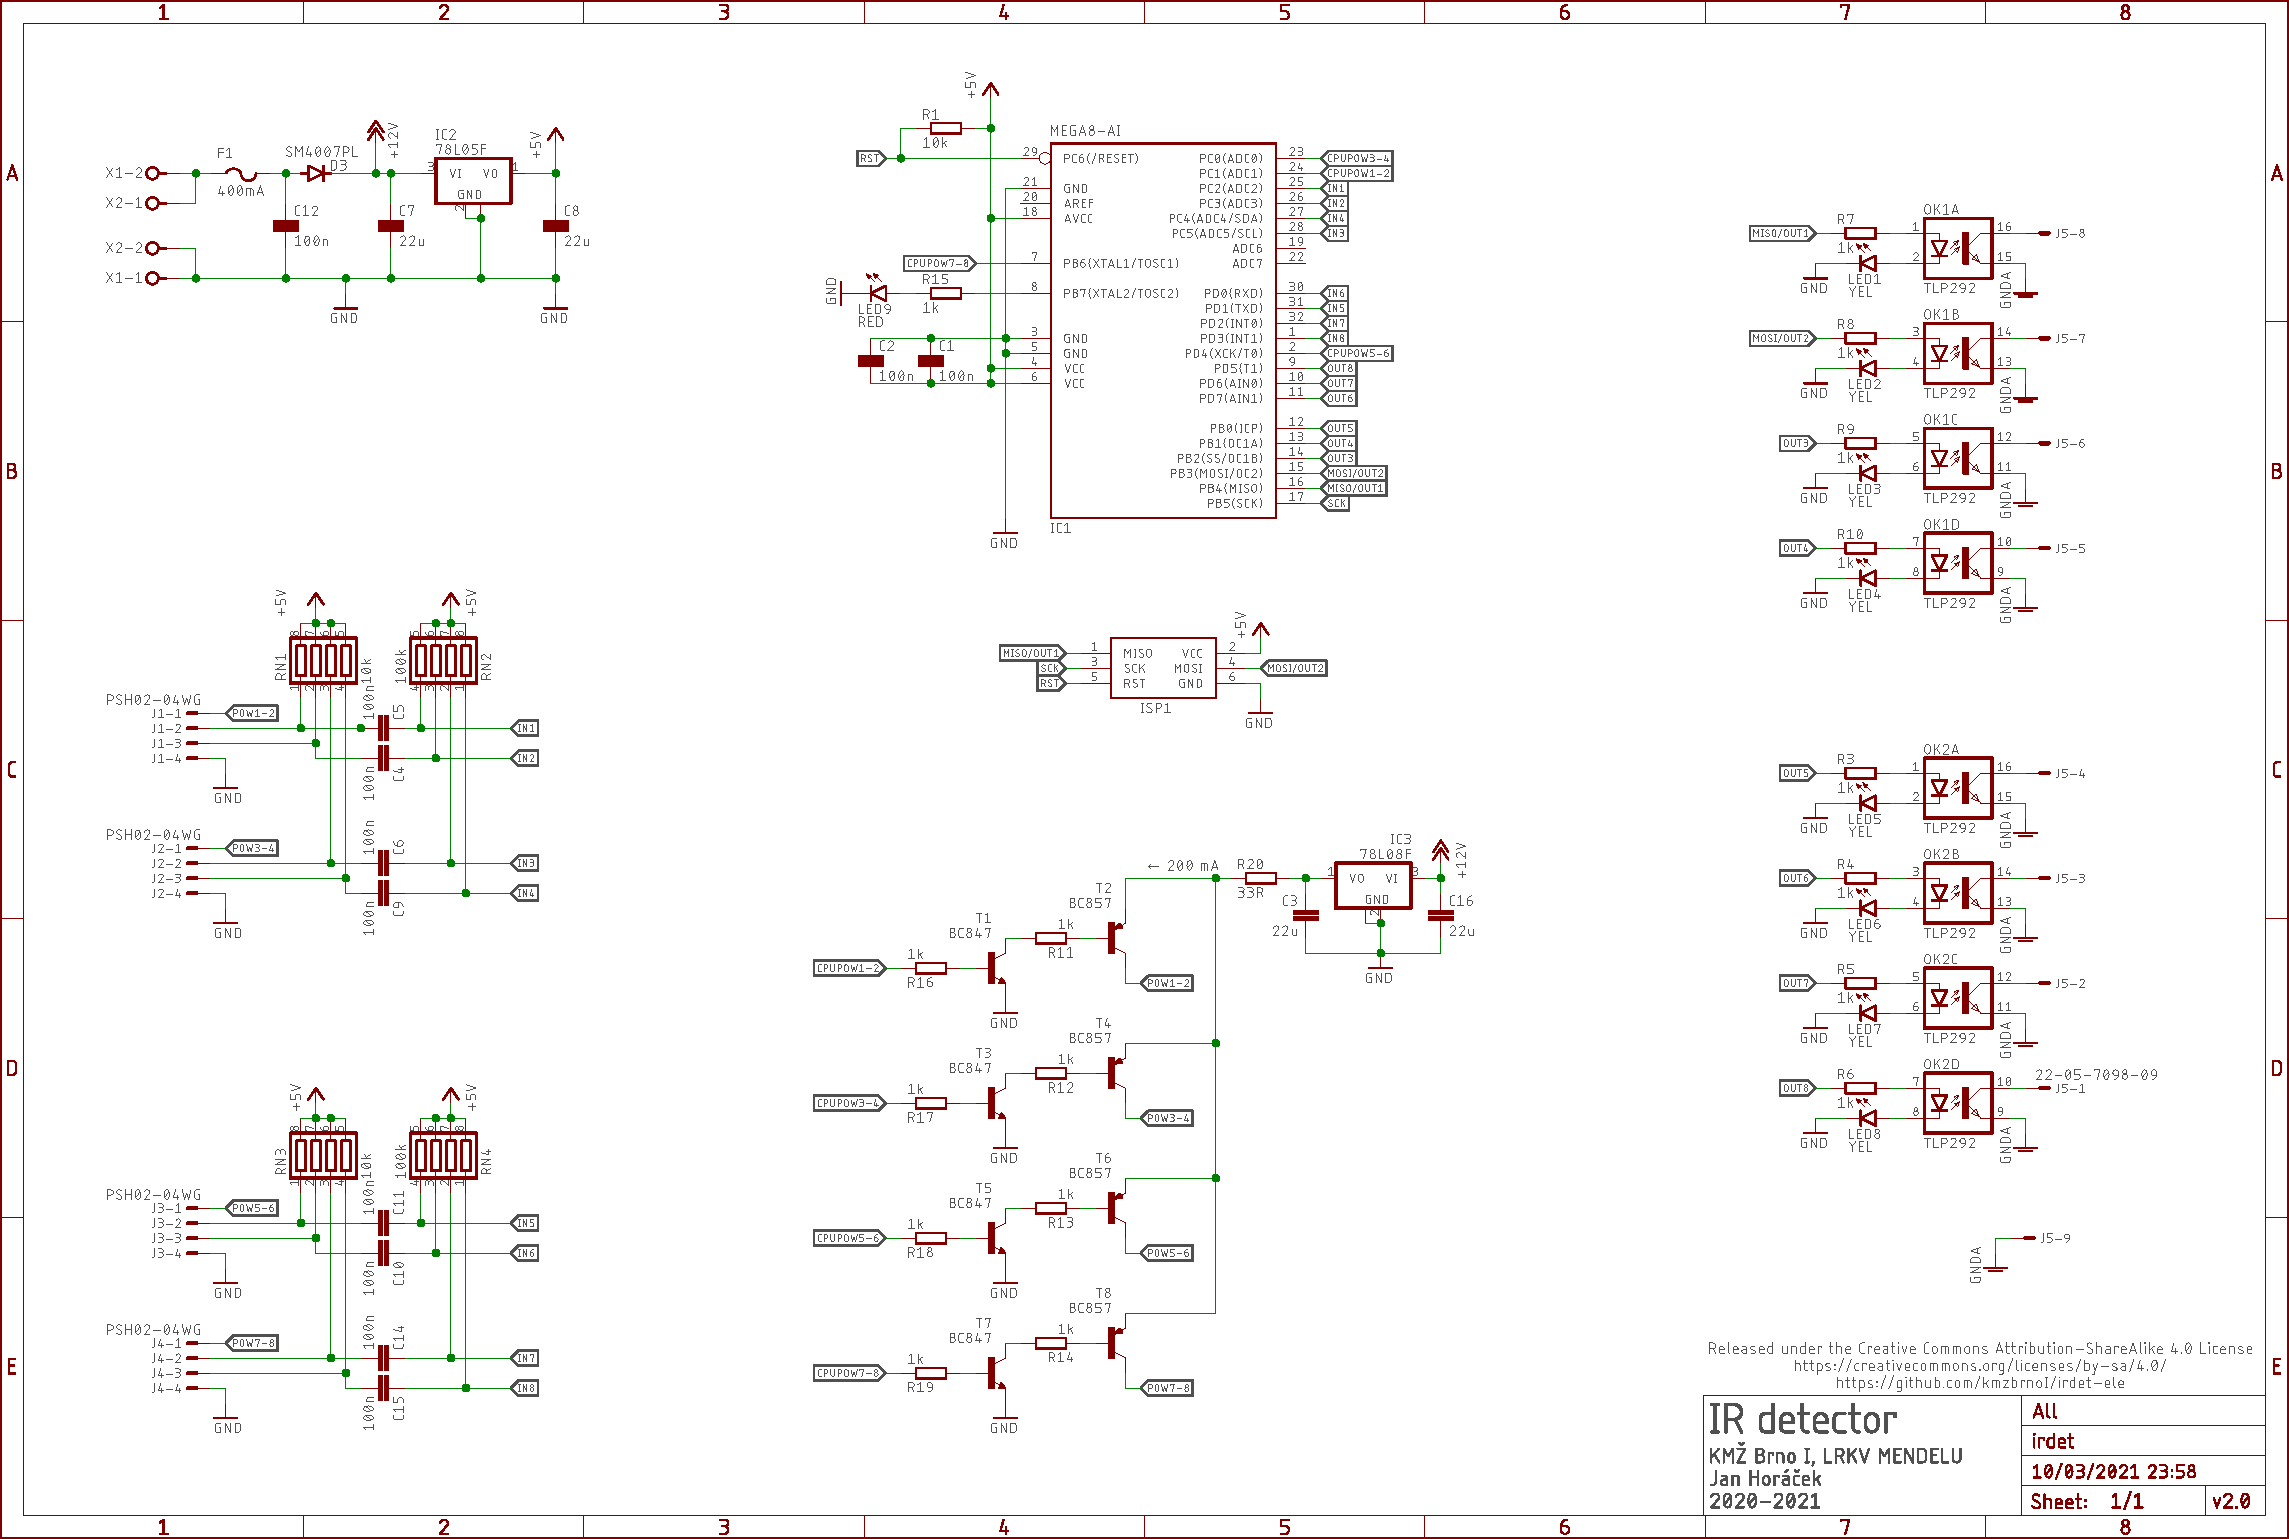
\includegraphics[angle=90,width=\textwidth]{data/irdet-ele.pdf}
\caption{Schéma desky \textit{IRdet}.}
\label{fig:irdet-sch}
\end{figure}


\end{document}
